%% $RCSfile: proj_proposal.tex,v $
%% $Revision: 1.3 $
%% $Date: 2016/06/10 03:44:08 $
%% $Author: kevin $

\documentclass[11pt, a4paper, twoside, openright]{report}

\usepackage{float} % lets you have non-floating floats
\usepackage{url} % for typesetting urls
\usepackage{wrapfig}
\usepackage[image,ecs]{vuwproject}

\renewcommand{\thesection}{\arabic{section}}

%  We don't want figures to float so we define
%
\newfloat{fig}{thp}{lof}[chapter]
\floatname{fig}{Figure}
\graphicspath{ {./Figures/} }

 

\title{Self Tuning Buck Converter}
\author{Niels Daniel Clayton}
\supervisor{Daniel Burmester}
\otherdegree{Honours of Electronic and Computer System Engineering}

\begin{document}

% Make the page numbering Roman, until after the contents, etc.
\frontmatter

%%%%%%%%%%%%%%%%%%%%%%%%%%%%%%%%%%%%%%%%%%%%%%%%%%%%%%%

\begin{abstract}
  This document gives some ideas about how to write a project
  proposal, and provides a template for a proposal. You should discuss
  your proposal with your supervisor.
\end{abstract}

%%%%%%%%%%%%%%%%%%%%%%%%%%%%%%%%%%%%%%%%%%%%%%%%%%%%%%%

\maketitle

%\tableofcontents

% we want a list of the figures we defined
%\listof{fig}{Figures}

%%%%%%%%%%%%%%%%%%%%%%%%%%%%%%%%%%%%%%%%%%%%%%%%%%%%%%%

\mainmatter

%%%%%%%%%%%%%%%%%%%%%%%%%%%%%%%%%%%%%%%%%%%%%%%%%%%%%%%

\section*{1. Introduction}


\subsection*{Switch Mode Power Supplies}

Switch mode power supplies convert a DC input voltage to another DC output voltage. They are commonly used in a wide variety of consumer and professional appliances such as laptops and chargers due to their high efficiency compared to other DC-to-DC converters. This project will 

The step-down switch mode power supply also known as a buck converter, is a common DC-to-DC power converter that steps down an input voltage to a desired output efficiently. Currently the design of these converters for specific applications requires a specifically designed output filter, designed around the switching speed of the converter. This filter will smooth the converter output voltage and maintain the inductor current ripple at the designed values. However this design process is not always applicable, if the specified components for the filter are not available there can be lead times, cost implications and delays.

\begin{figure}[h!]
  \begin{center}
    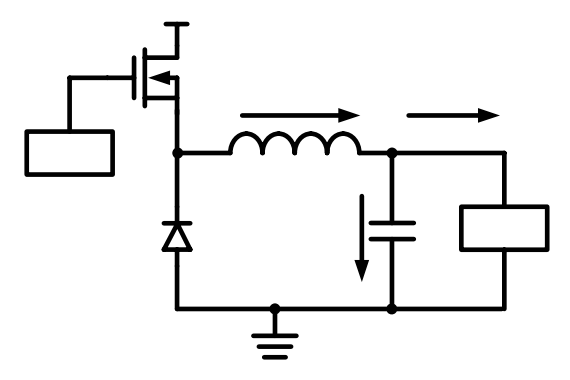
\includegraphics[width=0.6\linewidth]{asynchronous_buck.png} 
    \caption{Asynchronous buck converter topology \cite{BuckTopology}}
    \label{asynchronous_buck}
  \end{center}
\end{figure} 

This project aims to remove the need for designing the output stage of the buck converter. Using a control system, the switching frequency and duty cycle of the converter can be modulated to meet a selected inductor ripple, while maintaining a selected output voltage. This project will focus on the design and implementation this control system on a basic asynchronous buck converter. 


\section*{2. The Problem}

In this section you should give a brief description of the problem
itself. You want to briefly explain the problem, why it is important
to solve the problem and define your project aims. After reading this
section, the reader should understand why it is a problem, believe
that it is important to solve and have a clear idea of the aims of your project.

When describing the aims of the project, you should avoid vague,
unmeasurable words like `analyse', `investigate', `describe', and use
specific, measurable words like `implement', `demonstrate', `show',
`prove'.

For example:

\begin{itemize}
\item[\bf Good] The aim of this project is to implement and evaluate a
  management system for network switches;
\end{itemize}
is much better than:
\begin{itemize}
\item[\bf Bad] The aim of this project is to investigate management
  systems for network switches.
\end{itemize}

In the second case there is no idea of how much work is involved, and
you will never know whether you have finished. You and your supervisor
(and the markers of your project) may have very different ideas about
what such an `investigation' involves. Of course, it is possible that
the task you set yourself is not achievable, but if you are clear from
the outset this is less likely, and will more easily be corrected.

\section*{3. Proposed Solution}

In this section you will explain how solve the problem, that is, how
you intend to carry the project out. At this early stage you need to
be both clear about what you are going to do and flexible enough to
adapt to changing circumstances. Making an early plan will not prevent
you from running into trouble, but it will help you identify possible
problems early. For example, if you intended to run an experiment in
HCI, you might realise early on that there would be problems gathering
sufficient data to get reliable results, and that you should re-design
your experiment.

Part of the planning process involves producing a timetable for when
the work is actually going to be done.

Each part of the project should produce some output. For example you
might plan on spending two weeks on background reading: the output of
this will be a bibliography, and a possibly a literature survey for
your report. Indeed, if you take the advice given above about having
specific, measurable goals, you should describe this part of your
project as:

\begin{itemize}
\item[\bf Good] Produce bibliography (est: 2 weeks)
\end{itemize}
rather than
\begin{itemize}
\item[\bf Bad] Background reading (est: 2 weeks)
\end{itemize}

Note that the methodology you outline here is dependent upon the type
of project and engineering area. You must talk to your supervisor
about this.

\section*{4. Evaluating your Solution}

In this section you will explain how you will evaluate your solution
once you have built it. The method of evaluation will be domain
specific. Your supervisor should provide guidance as to what is an
appropriate form of evaluation. For example, user testing for a HCI
project or performance measurement for a Network Engineering project.

\section*{5. Resource Requirements}

In this section you will detail any resource requirements such as
hardware, software or access to subjects.

%%%%%%%%%%%%%%%%%%%%%%%%%%%%%%%%%%%%%%%%%%%%%%%%%%%%%%%
\backmatter
%%%%%%%%%%%%%%%%%%%%%%%%%%%%%%%%%%%%%%%%%%%%%%%%%%%%%%%

\bibliographystyle{ieeetr}
\bibliography{sample}
\end{document}
